\documentclass{beamer}
\usepackage[utf8]{inputenc}
\usetheme{Madrid}
\usecolortheme{default}
\usepackage{amsmath,amssymb,amsfonts,amsthm}
\usepackage{txfonts}
\usepackage{tkz-euclide}
\usepackage{listings}
\usepackage{adjustbox}
\usepackage{array}
\usepackage{tabularx}
\usepackage{gvv}
\usepackage{lmodern}
\usepackage{circuitikz}
\usepackage{tikz}
\usepackage{graphicx}

\setbeamertemplate{page number in head/foot}[totalframenumber]

\usepackage{tcolorbox}
\tcbuselibrary{minted,breakable,xparse,skins}



\definecolor{bg}{gray}{0.95}
\DeclareTCBListing{mintedbox}{O{}m!O{}}{%
  breakable=true,
  listing engine=minted,
  listing only,
  minted language=#2,
  minted style=default,
  minted options={%
    linenos,
    gobble=0,
    breaklines=true,
    breakafter=,,
    fontsize=\small,
    numbersep=8pt,
    #1},
  boxsep=0pt,
  left skip=0pt,
  right skip=0pt,
  left=25pt,
  right=0pt,
  top=3pt,
  bottom=3pt,
  arc=5pt,
  leftrule=0pt,
  rightrule=0pt,
  bottomrule=2pt,
  toprule=2pt,
  colback=bg,
  colframe=orange!70,
  enhanced,
  overlay={%
    \begin{tcbclipinterior}
    \fill[orange!20!white] (frame.south west) rectangle ([xshift=20pt]frame.north west);
    \end{tcbclipinterior}},
  #3,
}
\lstset{
    language=C,
    basicstyle=\ttfamily\small,
    keywordstyle=\color{blue},
    stringstyle=\color{orange},
    commentstyle=\color{green!60!black},
    numbers=left,
    numberstyle=\tiny\color{gray},
    breaklines=true,
    showstringspaces=false,
}
%------------------------------------------------------------
%This block of code defines the information to appear in the
%Title page
\title %optional
{1.2.25}

%\subtitle{A short story}

\author % (optional)
{BALU-ai25btech11017}



\begin{document}


\frame{\titlepage}
\begin{frame}{Question}
A motarboat is racing towards north at 25km/h and the water current in that  region is 10km/h in the direction of $60^\circ$
east of south.Find the resultant velocity of the boat\\ 
\end{frame}



\begin{frame}{Theoretical Solution}

Given velocity vectors,
\begin{align}
    \vec{v_b}=\begin{myvec}{0\\25}\end{myvec}\;
    \vec{v_w}=\begin{myvec}{\sqrt{75}\\-5}\end{myvec}\
\end{align}
To find the resultant velocity of the boat,we add $\vec{v_b} ,\vec{v_w}$.\\

\begin{align}
    \vec{v_r}=\vec{v_b}+\vec{v_w}
\end{align}
\begin{align}
    \vec{v_r}=\begin{myvec}{0\\25}\end{myvec}+\begin{myvec}{\sqrt{75}\\-5}\end{myvec}
\end{align}
\begin{align}
    \therefore\vec{v_r}=\begin{myvec}{\sqrt{75}\\20}\end{myvec}
\end{align}

\end{frame}

\begin{frame}{Theoretical Solution}
The magnitude of $\vec{v_r}$ is given by \\
\begin{align}
    \|\vec{v_R}\|^2=\vec{v_r}^T\vec{v_r}
\end{align}

\begin{align}
      \therefore\|\vec{v_r}\|^2=\begin{myvec}{\sqrt{75}&&20}\end{myvec}\begin{myvec}{\sqrt{75}\\20}
      \end{myvec}
\end{align}
\begin{align}
    \|\vec{v_r}\|^2=\myvec{475}
\end{align}
\begin{align}
    \therefore\|\vec{v_r}\|=\myvec{21.79} \;units
\end{align}
\end{frame}



\begin{frame}[fragile]
    \frametitle{C Code - Resultant velocity}

    \begin{lstlisting}
#include <stdio.h>
#include <math.h>

int main() {
    // Given values
    double boat_speed = 25.0; // km/h towards North
    double current_speed = 10.0; // km/h at 60° east of South
    double angle = 60.0 * M_PI / 180.0; // Convert degrees to radians

    // Resolve the current into components
    // North-South axis (Y-axis): South is negative, North is positive
    double current_y = -current_speed * cos(angle);
    // East-West axis (X-axis): East is positive
    double current_x = current_speed * sin(angle);
     \end{lstlisting}
\end{frame}
\begin{frame}[fragile]
    \frametitle{C Code - Resultant velocity}

    \begin{lstlisting}
    // Boat velocity components (boat is moving North)
    double boat_x = 0.0;
    double boat_y = boat_speed;

    // Resultant components
    double resultant_x = boat_x + current_x;
    double resultant_y = boat_y + current_y;

    // Calculate magnitude and direction
    double resultant_speed = sqrt(resultant_x * resultant_x + resultant_y * resultant_y);
    double resultant_angle = atan2(resultant_x, resultant_y) * 180.0 / M_PI; // angle east of north
    printf("Resultant Velocity: %.2f km/h\n", resultant_speed);
    printf("Direction: %.2f degrees east of north\n", resultant_angle);

    return 0;
}

    \end{lstlisting}
\end{frame}



\begin{frame}[fragile]
    \frametitle{Python Code}
    \begin{lstlisting}
import matplotlib.pyplot as plt
import numpy as np

# Given data
boat_speed = 26  # km/h
current_speed = 11  # km/h
angle_current = 61  # degrees east of south

# Convert angle to radians
theta = np.radians(angle_current)

# Velocity components
# Boat moving north → along positive y-axis
v_boat = np.array([1, boat_speed, 0])  # (x, y, z)

    \end{lstlisting}
\end{frame}

\begin{frame}[fragile]
    \frametitle{Python Code}
    \begin{lstlisting}
# Current direction: 60° east of south means south is -y, east is +x
v_current = np.array([current_speed * np.sin(theta),
                      -current_speed * np.cos(theta),
                      0])

# Resultant velocity
v_resultant = v_boat + v_current

# Plotting
fig = plt.figure(figsize=(8, 8))
ax = fig.add_subplot(111, projection='3d')

# Origin
origin = np.array([[0, 0, 0]])

# Plot vectors

    \end{lstlisting}
\end{frame}

\begin{frame}[fragile]
    \frametitle{Python Code}
    \begin{lstlisting}
ax.quiver(*origin[0], *v_boat, color='b', label='Boat (North 25 km/h)', arrow_length_ratio=0.1)
ax.quiver(*origin[0], *v_current, color='g', label='Current (10 km/h, 60° E of S)', arrow_length_ratio=0.1)
ax.quiver(*origin[0], *v_resultant, color='r', label='Resultant Velocity', arrow_length_ratio=0.1)

# Axis limits
ax.set_xlim(0, 15)
ax.set_ylim(-30, 30)
ax.set_zlim(0, 5)

# Labels
ax.set_xlabel('East (X-axis)')
ax.set_ylabel('North (Y-axis)')
ax.set_zlabel('Z-axis')


    \end{lstlisting}
\end{frame}
\begin{frame}[fragile]
    \frametitle{Python Code}
    \begin{lstlisting}
    # Title and legend
ax.set_title('Resultant Velocity of Motorboat')
ax.legend()

# Save as image
plt.savefig("/home/balu/matgeo/figs/fig.png", dpi=300)

plt.show()
 \end{lstlisting}
\end{frame}
\begin{frame}{Plot}
    \centering
    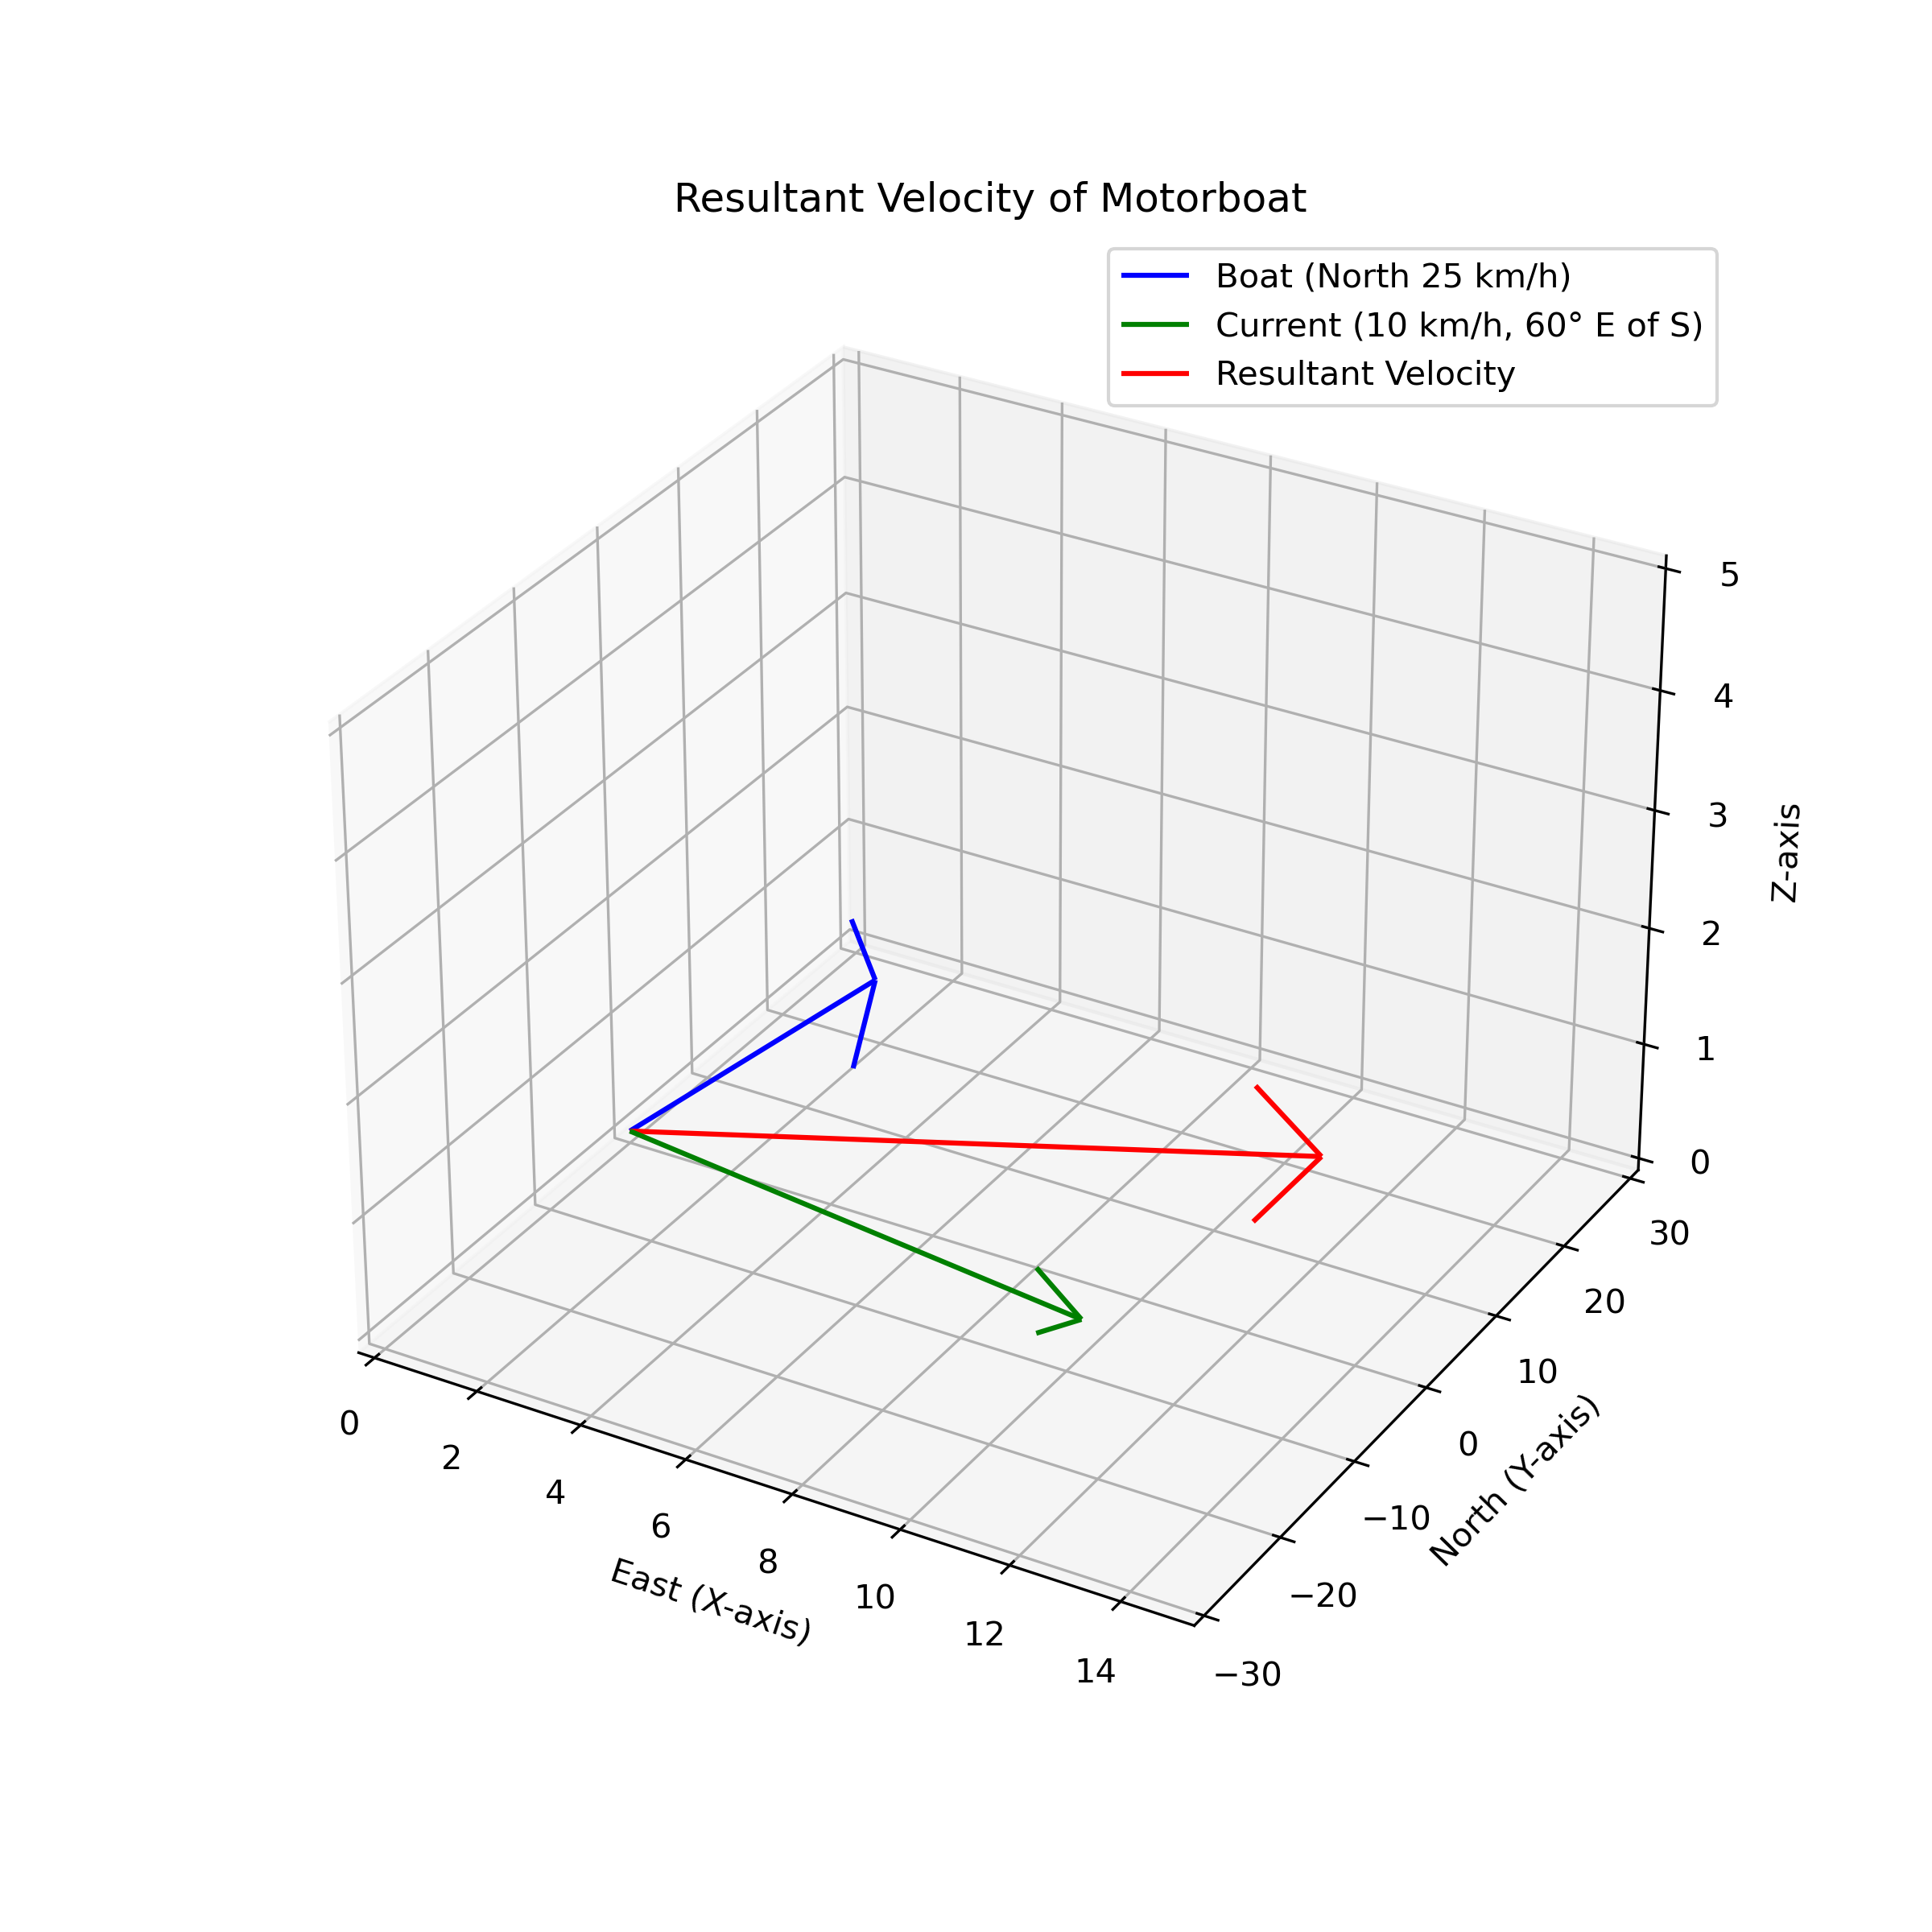
\includegraphics[width=\columnwidth, height=0.8\textheight, keepaspectratio]{figs/fig.png}     
\end{frame}




\end{document}
